\documentclass[]{article}	% 这里可以设置文字样式

\usepackage[UTF8]{ctex}	% 中文语言包
\usepackage[shortlabels]{enumitem}	% 编号扩展功能包
\usepackage{graphicx}	% 图片功能包
\usepackage{subfigure}	% 子图功能包
\usepackage{booktabs}	% 表格功能包
\usepackage{multirow}	% 合并多行表格
\usepackage{amsmath}	% 公式功能包
%\usepackage{caption}	% 暂时未用到
%\usepackage{listings}	% 暂时未用到
%\usepackage{lineno}	% 为每一行文字编号,暂时未用到
%\usepackage{setspace}	% 暂时未用到

%*****************************************************
%			伪代码
\usepackage{algorithm}
\usepackage{algorithmicx}
\usepackage{algpseudocode}

\floatname{algorithm}{算法}
\renewcommand{\algorithmicrequire}{\textbf{输入:}}
\renewcommand{\algorithmicensure}{\textbf{输出:}}
%*****************************************************

\title{\LaTeX 排版入门的正确姿势}
\author{碎金}

\begin{document}

\maketitle	% 生成封面
\thispagestyle{empty}	% 设置该页页眉页脚格式
\clearpage	% 插入空白页

\setcounter{page}{1}	% 重置该页的页码
\pagenumbering{roman}	% 设置该页的页码格式

\begin{abstract}	% 文字直接在创建好的环境中输入就可以了。编译后就可以看到效果。

这里可以写你的摘要。\LaTeX 是一个很好用的排版工具,常常用在学术论文的排版上。优点是排版成果美观,功能强大。缺点是入门门槛相对较高,学习曲线陡峭,不是所见即所得的排版工具。

\end{abstract}

\clearpage
\tableofcontents
\clearpage

\setcounter{page}{1}
\pagenumbering{arabic}

\section{基础介绍}
\label{sec.intro}

视频的时间目录见表\ref{tab.tableoftimecontents}所示:
\begin{table}[htbp]
	\centering
	\caption{视频的时间目录}
	\begin{tabular}{rll}
		\toprule
		编号 & 内容 & 时间 \\
		\midrule
		1     & LaTeX简介 & 00分32秒 \\
		2     & 编译器的简单配置 & 04分05秒 \\
		3     & 新建文件及其基本认识 & 04分49秒 \\
		4     & 创建目录  & 10分53秒 \\
		5     & 页码的设置 & 12分06秒 \\
		6     & 基础操作的学习(交叉引用等等) & 15分04秒 \\
		7     & 如何插入图片 & 19分51秒 \\
		8     & 如何快速生成eps文件 & 26分38秒 \\
		9     & 如何插入表格 & 28分54秒 \\
		10    & 公式的输入 & 33分03秒 \\
		11    & 文献及其引用 & 41分56秒 \\
		12    & 结尾    & 46分38秒 \\
		\bottomrule
	\end{tabular}%
	\label{tab.tableoftimecontents}%
\end{table}%

\subsection{基操}
\label{sec.intro.jicao}

\paragraph{如何引用?}  % 使用\paragraph不会编号

使用命令\textbackslash ref\{\}以及在需要被引用的地方使用\textbackslash label\{\}。

\LaTeX 换行需要在编译器中中间空一行。

\paragraph{如何列举?}

方法1:
\begin{itemize}
	\item 第一个
	\item 第二个
	\item 第三个
\end{itemize}

方法2(带编号):
\begin{enumerate}[(1).]
	\item 哈
	\item 嘿
\end{enumerate}

\clearpage
\section{如何插入图片?}

插入单张图片可以直接从文件夹中拖拽到编译器中,或者对文件复制,粘贴到编译器中。
\begin{figure}[htbp]
	\centering
	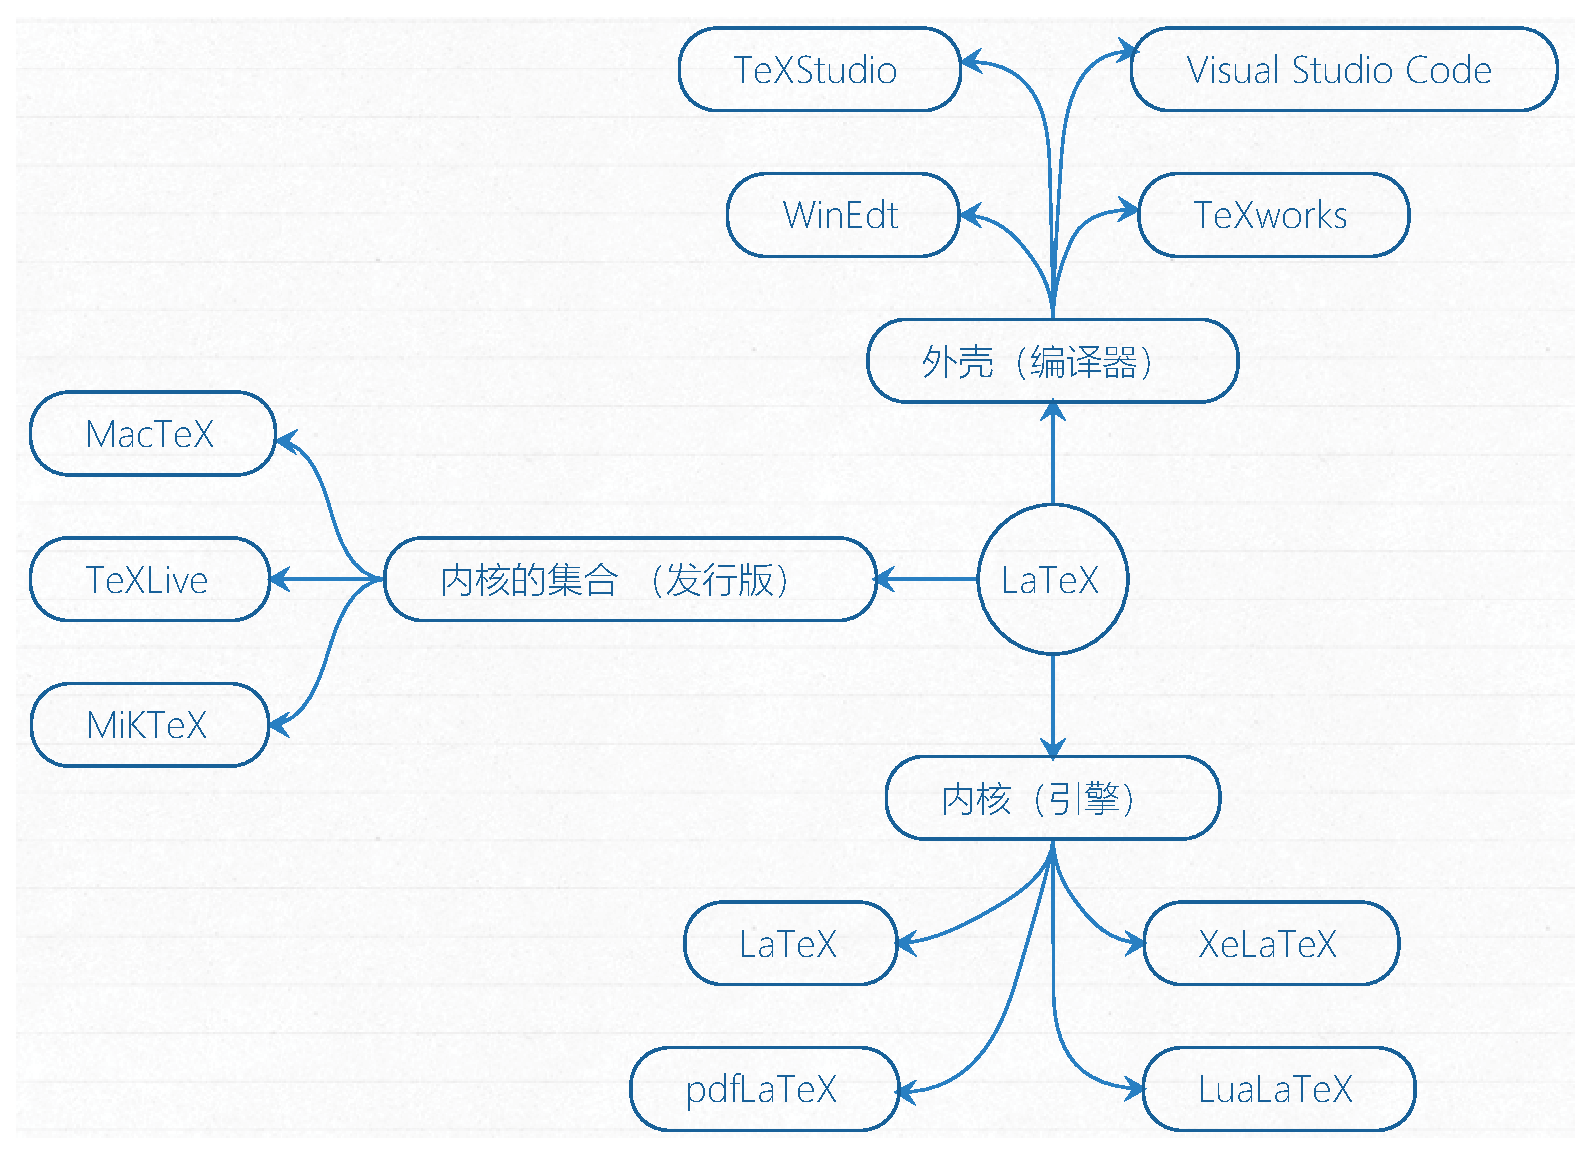
\includegraphics[width=1\linewidth]{Figures/Figure1_LaTeXIntro}
	\caption{\LaTeX 的说明示意图。}
	\label{fig:figure1latexintro}
\end{figure}

插入子图可以复制下面的模板代码,修改各个子图的属性(例如比例、图片路径)。这里我展示了引用图\ref{fig:sub1}、图\ref{fig:subfigure}的效果。
\begin{figure}[htbp]
	\centering
	\subfigure[子图\#1]
	{
		\label{fig:sub1}		
		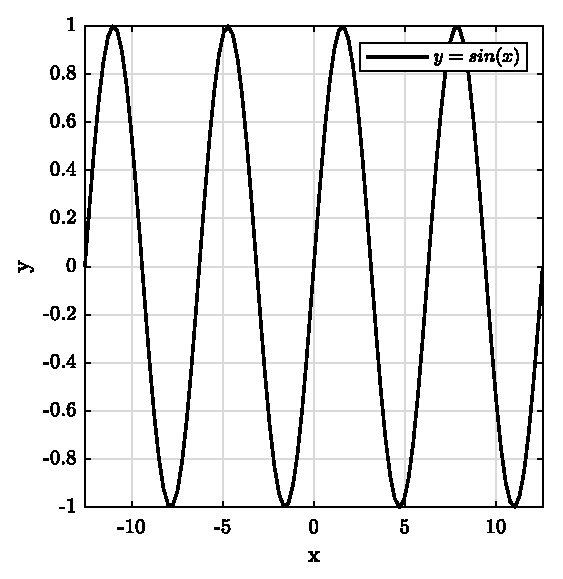
\includegraphics[width=0.45\textwidth]{Figures/Subfigure_1.eps}
	}
	\subfigure[子图\#2]
	{
		\label{fig:sub2}		
		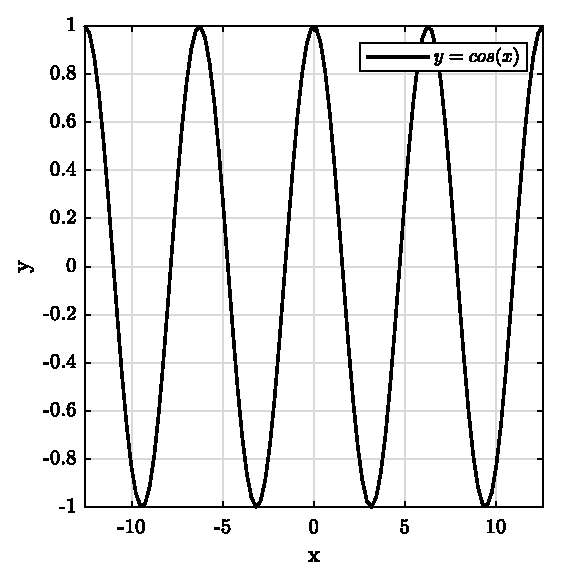
\includegraphics[width=0.45\textwidth]{Figures/Subfigure_2.eps}
	}
	\subfigure[子图\#3]
	{
		\label{fig:sub3}		
		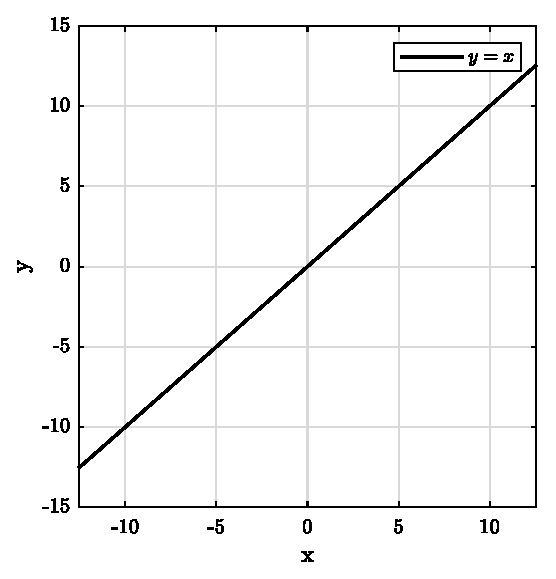
\includegraphics[width=0.45\textwidth]{Figures/Subfigure_3.eps}
	}
	\subfigure[子图\#4]
	{
		\label{fig:sub4}		
		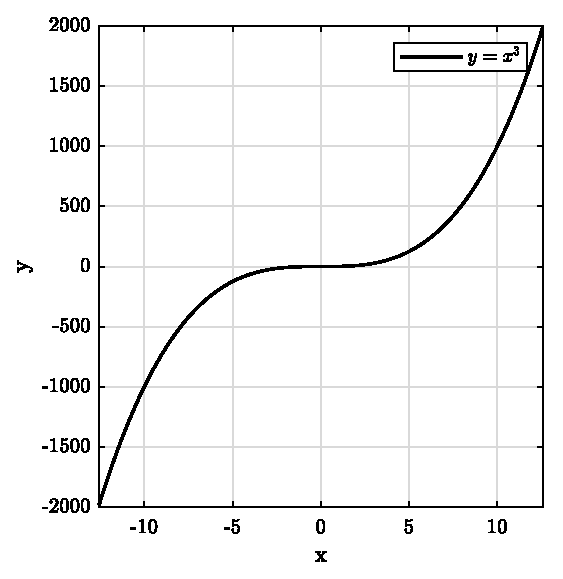
\includegraphics[width=0.45\textwidth]{Figures/Subfigure_4.eps}
	}
	\caption{这里是子图(subfigure)的示例。}
	\label{fig:subfigure}
\end{figure}

\clearpage
\section{如何插入表格?}

利用Excel的插件``Excel2latex''来插入表格,效果见表\ref{tab.1}和表\ref{tab.2}。
\begin{table}[htbp]
	\centering
	\caption{示例表格1。}
	\begin{tabular}{rrrr} % r:向右对齐; c:居中对齐; l:向左对齐。 这个表格有4列,每个字母控制一列。
		\multicolumn{4}{l}{表格首行} \\	% \multicolumn{4}{l}{}合并了4列表格并把文字向左对齐
		编号    & x     & y     & z \\	% &为对齐符号
		1     & 0.553225 & 0.472727 & 0.219954 \\	% \\为换行符号
		2     & 0.65798 & 0.699449 & 0.050294 \\
		3     & 0.941575 & 0.570867 & 0.699262 \\
	\end{tabular}%
	\label{tab.1}%
\end{table}%

\begin{table}[htbp]
	\centering
	\caption{示例表格2。}
	\begin{tabular}{|c|c|c|c|}
		\toprule 
		\multicolumn{4}{|c|}{表格首行} \\
		\midrule
		编号    & x     & y     & z \\
		\midrule
		1     & 0.553225 & 0.472727 & 0.219954 \\
		\midrule
		2     & 0.65798 & 0.699449 & 0.050294 \\
		\midrule
		3     & 0.941575 & 0.570867 & 0.699262 \\
		\bottomrule
	\end{tabular}%
	\label{tab.2}%
\end{table}%

\clearpage
\section{公式}	% 需要用到宏包amsmath

\subsection{公式的输入}

TeXstudio创建公式环境的快捷键:Ctrl+Shift+N:
\begin{equation}\label{eq.1}
	y = \int_{0}^{1} x dx^{2}_{a}
\end{equation}
公式也可以被引用,见公式\eqref{eq.1}。

上标快捷键:Ctrl+Shift+U
下标快捷键:Ctrl+Shift+D

TeXstudio创建行内公式环境的快捷键:Ctrl+Shift+M。例如这样的公式$ TSR=\dfrac{\Omega r}{U_{w}} $就没有编号。

\subsection{公式组}

多个公式应该使用\textbackslash begin\{align\},如下:
\begin{align}
	m & = x + y + z + 1 \\
	n & = 2x - y + 3z \\
	r & = 5x + z \\
	3124312 + 541421 & = ?
\end{align}

如果想加个大的花括号则要在equation环境中嵌套aligned,如下:
\begin{equation}
	\left\{
	\begin{aligned}
		m & = x + y + z + 1 \\
		n & = 2x - y + 3z \\
		r & = 5x + z
	\end{aligned}
	\right.
\end{equation}


\subsection{公式换行}

%有的公式太长需要换行,也可以用equation环境中嵌套aligned来实现,如下:
%\begin{equation}
%	\begin{aligned}
%	a = & b + c + d + e + \\
%	& f + g + h + i + j + \\
%	& k + l
%	\end{aligned}
%\end{equation}


有的公式需要递推换行,也可以用equation环境中嵌套aligned来实现,如下:
\begin{equation}
	\begin{aligned}
		a = & b + c + d + e + \\
		  = & f + g + h + i + j + \\
		  = & k + l\ddots
	\end{aligned}
\end{equation}

\section{文献及引用}

最基础的引用方式是\textbackslash cite\{\}, 其他方式有:\textbackslash citet\{\},\textbackslash citep\{\}等等。

示例,文献见\cite{Davis1995Bose},\cite{Ertekin2014,Davis1995Bose}所示。



\newpage
\bibliographystyle{plain}	% 设置文献样式
\bibliography{ExampleBib}	% 设置文献的文件路径
\end{document}






\\
= &
-\frac{1}{m}\left[ \sum_{i=1}^{m} x_i \left(1\{y_i = j\}  - \sum_{j=1}^{k} 1\{y_i = j\} \frac{\exp(\theta_j^T x_i)}{\sum_{l=1}^{k}\exp(\theta_l^T x_i)} \right) \right] 




